\documentclass[11pt,a4paper]{article}
\usepackage[utf8]{inputenc}
\usepackage[T1]{fontenc}
\usepackage{lmodern}
\usepackage{geometry}
\geometry{
    a4paper,
    top=2.2cm,
    bottom=2.2cm,
    left=2.2cm,
    right=2.2cm
}

% Paketler
\usepackage{amsmath}
\usepackage{amssymb}
\usepackage{titlesec}
\usepackage{parskip}
\usepackage{setspace}
\setstretch{1.12}
\usepackage{tikz}
\usetikzlibrary{shapes.geometric, arrows.meta, positioning, calc}
\usepackage{hyperref}
\usepackage{enumitem}

% Başlık biçimlendirmesi (Örnek şablona birebir uyumlu)
\titleformat{\section}
  {\large\bfseries}{\thesection.}{0.5em}{}
\titlespacing*{\section}{0pt}{1.2ex plus .2ex minus .2ex}{0.5ex plus .1ex}

\titleformat{\subsection}
  {\normalsize\bfseries}{\thesubsection}{0.5em}{}
\titlespacing*{\subsection}{0pt}{1.0ex plus .2ex minus .2ex}{0.4ex plus .1ex}

\setlength{\parskip}{5pt plus 1pt minus 1pt}
\setlength{\parindent}{0pt}

\begin{document}

% ==========================================
% PROJE BAŞLIĞI VE ÖĞRENCİ BİLGİLERİ
% ==========================================
\begin{center}
    {\Large \textbf{Real-Time Violence Detection and Privacy-Compliant Security Alert System via Multimodal Dynamic Fusion}\par}
\end{center}

\vspace{0.8em}

{\normalsize
\begin{tabular}{@{}ll}
\textbf{Fatma Ceylin Ayçiçek} & B221202023 \\ % Öğrenci numaranızı giriniz
\textbf{Ayşe Zeynep Turan}   & B221202007 \\ % Öğrenci numaranızı giriniz
\textbf{Gökay Yılmaz}         & B231202056 \\ % Öğrenci numaranızı giriniz
\textbf{Mehmet Kerem Çay}     & B221202010    % Öğrenci numaranızı giriniz
\end{tabular}
\par}

\vspace{1.2em}

% ==========================================
% BÖLÜM 1: PROJE TANIMI VE AMACI
% ==========================================
\section{PROJECT DESCRIPTION AND OBJECTIVE}

\subsection{Introduction}
% [İÇERİK NOTU]: Modern kamu güvenliği sistemlerinde video gözetimi ve derin öğrenmenin rolünü,
% gerçek zamanlı şiddet tespitinin neden kritik olduğunu bu kısımda açıklayınız.
In contemporary public security systems, automated surveillance has emerged as an essential requirement for proactive threat mitigation and rapid emergency response in crowded areas such as transit hubs, campuses, and city centers. Manual surveillance across hundreds of closed-circuit television (CCTV) cameras suffers from severe cognitive overload and human latency, frequently resulting in delayed interventions during violent outbreaks. This project introduces an edge-compatible, multimodal deep learning framework that unifies human skeleton tracking, dangerous object detection, and event-triggered acoustic verification to achieve real-time violence detection and low-latency security dispatch.

\subsection{Problem Analysis and Motivation}
% [İÇERİK NOTU]: Literatürdeki mevcut eksiklikleri (tek modlu sistemler, duruş ve nesne entegrasyonu eksikliği,
% yüksek gecikme, ses-görüntü senkronizasyonu ve sürekli dinleme kaynaklı KVKK/etik ihlallerini) vurgulayınız.
Current automated violence detection solutions are predominantly single-modal, relying solely on standard RGB video streams. These architectures exhibit significant failure modes in complex environments: they fail to distinguish playful physical interactions from genuine assaults, suffer severe performance degradation under low illumination, and cannot reliably detect concealed or small dangerous weapons (e.g., knives, firearms). Furthermore, while incorporating ambient audio can resolve visual ambiguities, continuous audio monitoring introduces grave legal and ethical infringements regarding personal data privacy regulations (such as GDPR and KVKK). Conventional multi-stream models also incur excessive latency ($>1.5\text{ s}$), rendering them unsuitable for urgent field intervention where sub-second alerts are mandatory.

\subsection{Project Goals and Expected Contributions}
% [İÇERİK NOTU]: Projenin somut hedeflerini (F1 > %90, <500 ms yanıt süresi, FPS >= 20, 
% olay tetikli ses dinlemesi ve mobil bildirim mekanizmasını) akademik bir üslupla ifade ediniz.
The primary objective of this project is to develop an end-to-end, privacy-compliant, multimodal violence detection and alerting platform operating at $\ge 20\text{ FPS}$ with an end-to-end response latency below $500\text{ ms}$. Key contributions of the proposed system include:
\begin{itemize}[leftmargin=*,noitemsep,topsep=2pt]
    \item \textbf{Synergistic Visual Analysis:} Coupling MediaPipe BlazePose coordinate extraction with LSTM temporal networks to model velocity and acceleration, combined with real-time YOLOv10 object detection for weapon identification.
    \item \textbf{Privacy-Preserving (Event-Triggered) Audio:} Activating microphone listening for only 5 seconds upon detecting an elevated visual violence probability ($\ge 60\%$), fully complying with data privacy mandates.
    \item \textbf{Dynamic Attention Fusion:} Implementing a Transformer-based attention mechanism that dynamically weights spatial pose, motion dynamics, object presence, and acoustic spectro-temporal features to produce reliable alarm decisions ($F_1 \ge 0.90$).
    \item \textbf{Instant Security Dispatch:} Automatically generating geolocated, timestamped push notifications to field security personnel via a dedicated mobile interface upon incident confirmation ($\ge 75\%$).
\end{itemize}

\newpage
% ==========================================
% BÖLÜM 2: SİSTEM MİMARİSİ VE TASARIMI (SAYFA 2)
% ==========================================
\section{SYSTEM ARCHITECTURE AND DESIGN}

\subsection{General Architecture}
% [İÇERİK NOTU]: Sistem mimarisini Girdi (Input), İşleme (Process) ve Çıktı (Output) olmak üzere
% üç ana katmanda açıklayınız.
The proposed system is structured around a high-throughput, modular pipeline divided into three cohesive layers: Input, Processing, and Output. The Input Layer captures live RTSP video feeds from surveillance cameras along with temporal metadata. The Processing Layer forms the multimodal inference engine, executing parallel visual extraction, conditional audio acquisition, and Transformer-driven feature fusion. The Output Layer delivers structured alerts, telemetry, and automated security reports.

\vspace{0.4em}

% MİMARİ AKIŞ DİYAGRAMI (Input -> Process -> Output)
\begin{center}
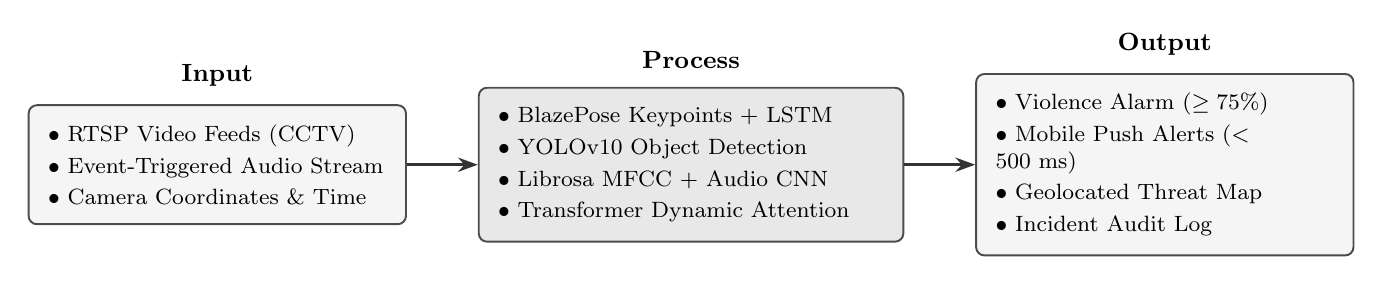
\begin{tikzpicture}[
    box/.style={
        draw=black!70,
        rounded corners=3pt,
        align=left,
        inner sep=7pt,
        font=\footnotesize,
        line width=0.7pt
    },
    titlebox/.style={
        font=\small\bfseries,
        align=center,
        inner sep=2pt
    },
    arrow/.style={
        -{Stealth[length=2.5mm, width=1.8mm]},
        line width=1.0pt,
        draw=black!80
    }
]

% Input Box
\node[box, fill=gray!8, text width=4.3cm] (inBox) {
    $\bullet$ RTSP Video Feeds (CCTV)\\[2pt]
    $\bullet$ Event-Triggered Audio Stream\\[2pt]
    $\bullet$ Camera Coordinates \& Time
};
\node[titlebox, above=0.15cm of inBox] (inTitle) {Input};

% Process Box
\node[box, right=0.9cm of inBox, fill=gray!18, text width=4.9cm] (procBox) {
    $\bullet$ BlazePose Keypoints + LSTM\\[2pt]
    $\bullet$ YOLOv10 Object Detection\\[2pt]
    $\bullet$ Librosa MFCC + Audio CNN\\[2pt]
    $\bullet$ Transformer Dynamic Attention
};
\node[titlebox, above=0.15cm of procBox] (procTitle) {Process};

% Output Box
\node[box, right=0.9cm of procBox, fill=gray!8, text width=4.3cm] (outBox) {
    $\bullet$ Violence Alarm ($\ge 75\%$)\\[2pt]
    $\bullet$ Mobile Push Alerts ($<500\text{ ms}$)\\[2pt]
    $\bullet$ Geolocated Threat Map\\[2pt]
    $\bullet$ Incident Audit Log
};
\node[titlebox, above=0.15cm of outBox] (outTitle) {Output};

% Arrows
\draw[arrow] (inBox.east) -- (procBox.west);
\draw[arrow] (procBox.east) -- (outBox.west);

\end{tikzpicture}
\end{center}

\vspace{0.4em}

Together, these modular layers establish a deterministic, fault-tolerant processing pipeline that transforms raw surveillance multimedia into rapid, actionable security intelligence without violating individual privacy rights.

\subsection{Data Management and Technological Infrastructure}
% [İÇERİK NOTU]: Arka uç, derin öğrenme çatıları, veritabanı, donanım ve dağıtım teknolojilerini bu kısımda belirtiniz.
The platform is designed to operate on a hybrid edge-cloud infrastructure to ensure ultra-low inference latency and high system availability. Data ingestion and real-time streaming pipelines are powered by OpenCV, FFmpeg, and Python 3.10+, orchestrated through a high-performance FastAPI asynchronous backend service.

Deep learning components are developed using PyTorch and ONNX Runtime for hardware-accelerated inference. Visual pose estimation utilizes MediaPipe BlazePose to track 33 kinematic landmarks, processed by an LSTM network to capture instantaneous velocity and acceleration vectors. Real-time weapon detection is executed via YOLOv10 (leveraging NMS-free dual assignments for sub-15 ms latency). Audio features are extracted using Librosa (Mel-Frequency Cepstral Coefficients - MFCC) and classified through an acoustic CNN/Transformer model running on parallel execution threads to prevent visual pipeline stalls. A cross-modal Transformer attention module dynamically integrates these intermediate representations to make the final classification decision.

Model training, cross-validation (5-fold), and domain adaptation are conducted across benchmark datasets including XD-Violence, RWF-2000, and UCF-Crime using CUDA-enabled GPU clusters (Google Colab and on-premise NVIDIA RTX environments). The backend state and audit logs are managed using PostgreSQL, with Redis utilized for fast session caching and event debouncing. Alert notifications are dispatched via WebSockets and Firebase Cloud Messaging (FCM) to a lightweight mobile application. The entire service stack is containerized using Docker and configured for scalable container deployment.

\end{document}
